% !TEX root =  master.tex
\chapter{Praktischer Teil}

\section{Umsetzung}
Die gewählte Datenbasis enthält alle Bundesliga-Spiele seit der Saison 2005/2006 mit
65+ Features. Während des Preprocessings wurde die Anzahl der Features durch
das Löschen nicht relevanter Features deutlich reduziert. Diese Features wurden dann
harmonisiert und mit einer Korrelationsmatrix auf ihre Aussagekraft geprüft.
Zur Verbesserung des Datensatzes wurden die aktuelle Form der Mannschaften (Elo) sowie Angriffs- und Verteidigungswerte errechnet. Um die Aussagekraft weiter zu erhöhen wurden außerdem Features eingeführt, die einen direkten Vergleich der Mannschaften ermöglichen.
Diese Features sind bspw. Differenzen der Elo und Angriffs- sowie Verteidigungswerte
oder die Anzahl der Punkte und Tore, die eine Mannschaft während der letzten Spiele erzielt hat.

\begin{figure}[H]
	
	\centering
	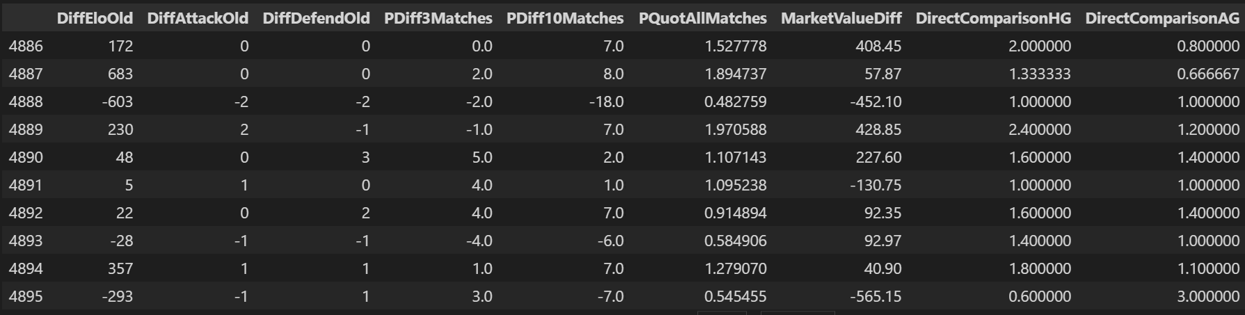
\includegraphics[scale=0.35]{\imagedir/Datensatz.png}
	\captionsetup{format=hang}
	\caption[Datensatz]{\label{fig:test}Datensatz.}
	
\end{figure}

Dadurch, dass die Zielvariablen bereits im Datensatz  vorliegen
handelt es sich um ein Supervised Learning-Problem. Dieses wurde
wie im Theorieteil erwähnt mit drei verschiedenen Methoden angegangen.
Dem Ensemble Learning, einem Neural Network sowie einem mathematischen Ansatz.

\section{Ergebnisse und Use Case-Validierung}
Angefangen beim Ensemble Learning erkennt man verschiedene Accuracys je Algorithmus. 
\begin{figure}[H]
	
	\centering
	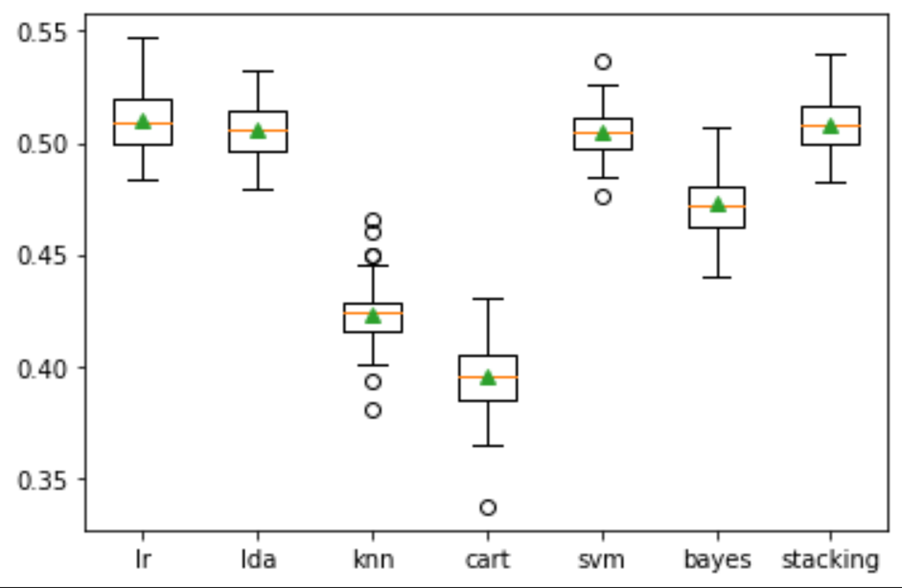
\includegraphics[scale=0.25]{\imagedir/Ensemble.png}
	\captionsetup{format=hang}
	\caption[Ensemble Learning]{\label{fig:test}Ensemble Learning.}
	
\end{figure}
Hierbei sind die Logistic Regression und Linear Discriminant Analysis am Besten. Das Stacking Modell welches alle Modelle vereint schneidet auch gut ab. Alle drei liegen bei einer Accuracy von etwas über 50\%}. Bei Betrachtung des Neural Networks fällt auf, dass die Accuracy
schon nach wenigen Epochen auf etwas unter 50\% konvergiert.
\begin{figure}[H]
	
	\centering
	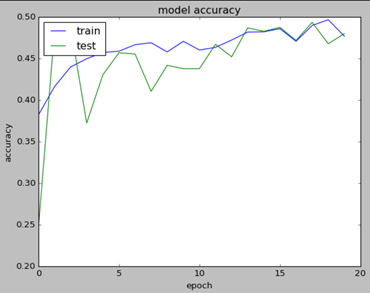
\includegraphics[scale=0.55]{\imagedir/NeuralNetwork.png}
	\captionsetup{format=hang}
	\caption[Neural Network]{\label{fig:test}Neural Network.}
	
\end{figure}
Nach einer Random Parameter Search konnte diese auf 53\% angehoben werden. Zuletzt haben wir mit der Poisson-Verteilung des mathematischen Ansatzes eine Accuracy von
etwa 50 Prozent erreicht. Die Angaben der Quelle konnten somit nicht validiert werden.

Um zu testen, wie gut das Modell unter Realbedingungen funktioniert
wurden im Verlauf der Saison 2021/22 Wetten simuliert. Für die
Simulation wurden die Predictions des Modells mit den Predictions von
vier verschiedenen Wettanbietern verglichen. Um die Predictions der
Wettanbieter zu erhalten wurde zuerst der Durchschnitt der Odds der
Wettanbieter für jedes Ereignis (Sieg Heimteam, Unentschieden, Sieg Auswärtsteam)
ermittelt. Dieser Durchschnitt wurde dann in eine Prozentzahl umgewandelt
und nach dem Maximum gefiltert um eine Prediction für jeden Spieltag zu erhalten.
Um auf die Predictions zu setzen mussten diese einen gewissen Schwellwert (XX\% Sicherheit) überschreiten.
Bei Überschreitung des Schwellwerts wurde je nach Höhe der \% Zahl ein bestimmter Betrag gewettet.
(Grafik wie viel ab welcher \% Zahl gewettet wird)

Auf die gesamte Saison 2021/22 betrachtet ergibt sich folgende Grafik.
\begin{figure}[H]
	
	\centering
	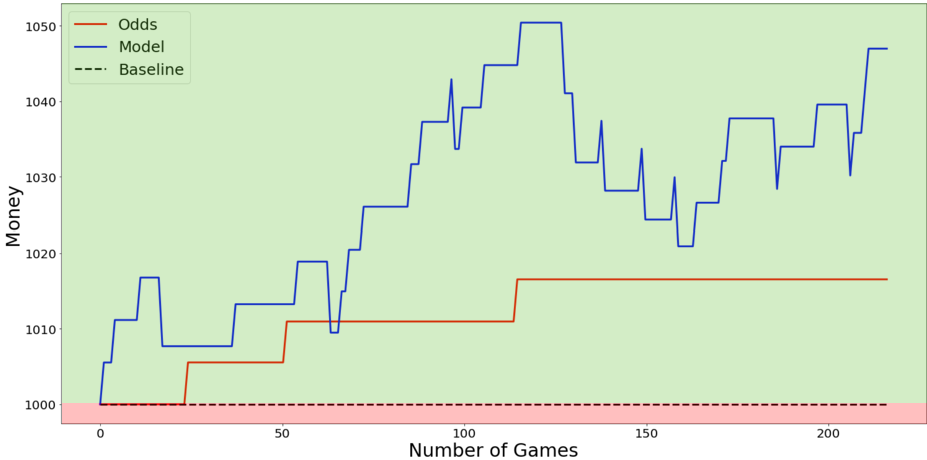
\includegraphics[scale=0.35]{\imagedir/Betting.png}
	\captionsetup{format=hang}
	\caption[Ensemble-Learning]{\label{fig:test}Betting.}
	
\end{figure}
Es lässt sich erkennen, dass das Modell am Ende der Saison zwar mehr Gewinn gemacht
hat, die Wettanbieter aber im Laufe der Saion besser performen. Auf die Bedeutung der Grafik
in Bezug auf den Business Use Case wird im Fazit genauer eingegangen.
